%% bare_conf.tex
%% V1.3
%% 2007/01/11
%% by Michael Shell
%% See:
%% http://www.michaelshell.org/
%% for current contact information.
%%
%% This is a skeleton file demonstrating the use of IEEEtran.cls
%% (requires IEEEtran.cls version 1.7 or later) with an IEEE conference paper.
%%
%% Support sites:
%% http://www.michaelshell.org/tex/ieeetran/
%% http://www.ctan.org/tex-archive/macros/latex/contrib/IEEEtran/
%% and
%% http://www.ieee.org/

%%*************************************************************************
%% Legal Notice:
%% This code is offered as-is without any warranty either expressed or
%% implied; without even the implied warranty of MERCHANTABILITY or
%% FITNESS FOR A PARTICULAR PURPOSE!
%% User assumes all risk.
%% In no event shall IEEE or any contributor to this code be liable for
%% any damages or losses, including, but not limited to, incidental,
%% consequential, or any other damages, resulting from the use or misuse
%% of any information contained here.
%%
%% All comments are the opinions of their respective authors and are not
%% necessarily endorsed by the IEEE.
%%
%% This work is distributed under the LaTeX Project Public License (LPPL)
%% ( http://www.latex-project.org/ ) version 1.3, and may be freely used,
%% distributed and modified. A copy of the LPPL, version 1.3, is included
%% in the base LaTeX documentation of all distributions of LaTeX released
%% 2003/12/01 or later.
%% Retain all contribution notices and credits.
%% ** Modified files should be clearly indicated as such, including  **
%% ** renaming them and changing author support contact information. **
%%
%% File list of work: IEEEtran.cls, IEEEtran_HOWTO.pdf, bare_adv.tex,
%%                    bare_conf.tex, bare_jrnl.tex, bare_jrnl_compsoc.tex
%%*************************************************************************

% *** Authors should verify (and, if needed, correct) their LaTeX system  ***
% *** with the testflow diagnostic prior to trusting their LaTeX platform ***
% *** with production work. IEEE's font choices can trigger bugs that do  ***
% *** not appear when using other class files.                            ***
% The testflow support page is at:
% http://www.michaelshell.org/tex/testflow/



% Note that the a4paper option is mainly intended so that authors in
% countries using A4 can easily print to A4 and see how their papers will
% look in print - the typesetting of the document will not typically be
% affected with changes in paper size (but the bottom and side margins will).
% Use the testflow package mentioned above to verify correct handling of
% both paper sizes by the user's LaTeX system.
%
% Also note that the "draftcls" or "draftclsnofoot", not "draft", option
% should be used if it is desired that the figures are to be displayed in
% draft mode.
%
\documentclass[10pt, conference, compsocconf]{IEEEtran}
%\documentclass[10pt]{IEEEtran}
\usepackage{times}

\usepackage{caption}
\captionsetup{font=footnotesize,justification=centering,labelsep=period}

% Add the compsoc option for Computer Society conferences.
%
% If IEEEtran.cls has not been installed into the LaTeX system files,
% manually specify the path to it like:
% \documentclass[conference]{../sty/IEEEtran}





% Some very useful LaTeX packages include:
% (uncomment the ones you want to load)


% *** MISC UTILITY PACKAGES ***
%
%\usepackage{ifpdf}
% Heiko Oberdiek's ifpdf.sty is very useful if you need conditional
% compilation based on whether the output is pdf or dvi.
% usage:
% \ifpdf
%   % pdf code
% \else
%   % dvi code
% \fi
% The latest version of ifpdf.sty can be obtained from:
% http://www.ctan.org/tex-archive/macros/latex/contrib/oberdiek/
% Also, note that IEEEtran.cls V1.7 and later provides a builtin
% \ifCLASSINFOpdf conditional that works the same way.
% When switching from latex to pdflatex and vice-versa, the compiler may
% have to be run twice to clear warning/error messages.






% *** CITATION PACKAGES ***
%
%\usepackage{cite}
% cite.sty was written by Donald Arseneau
% V1.6 and later of IEEEtran pre-defines the format of the cite.sty package
% \cite{} output to follow that of IEEE. Loading the cite package will
% result in citation numbers being automatically sorted and properly
% "compressed/ranged". e.g., [1], [9], [2], [7], [5], [6] without using
% cite.sty will become [1], [2], [5]--[7], [9] using cite.sty. cite.sty's
% \cite will automatically add leading space, if needed. Use cite.sty's
% noadjust option (cite.sty V3.8 and later) if you want to turn this off.
% cite.sty is already installed on most LaTeX systems. Be sure and use
% version 4.0 (2003-05-27) and later if using hyperref.sty. cite.sty does
% not currently provide for hyperlinked citations.
% The latest version can be obtained at:
% http://www.ctan.org/tex-archive/macros/latex/contrib/cite/
% The documentation is contained in the cite.sty file itself.






% *** GRAPHICS RELATED PACKAGES ***
%
\ifCLASSINFOpdf
  % \usepackage[pdftex]{graphicx}
  % declare the path(s) where your graphic files are
  % \graphicspath{{../pdf/}{../jpeg/}}
  % and their extensions so you won't have to specify these with
  % every instance of \includegraphics
  % \DeclareGraphicsExtensions{.pdf,.jpeg,.png}
\else
  % or other class option (dvipsone, dvipdf, if not using dvips). graphicx
  % will default to the driver specified in the system graphics.cfg if no
  % driver is specified.
  % \usepackage[dvips]{graphicx}
  % declare the path(s) where your graphic files are
  % \graphicspath{{../eps/}}
  % and their extensions so you won't have to specify these with
  % every instance of \includegraphics
  % \DeclareGraphicsExtensions{.eps}
\fi
% graphicx was written by David Carlisle and Sebastian Rahtz. It is
% required if you want graphics, photos, etc. graphicx.sty is already
% installed on most LaTeX systems. The latest version and documentation can
% be obtained at:
% http://www.ctan.org/tex-archive/macros/latex/required/graphics/
% Another good source of documentation is "Using Imported Graphics in
% LaTeX2e" by Keith Reckdahl which can be found as epslatex.ps or
% epslatex.pdf at: http://www.ctan.org/tex-archive/info/
%
% latex, and pdflatex in dvi mode, support graphics in encapsulated
% postscript (.eps) format. pdflatex in pdf mode supports graphics
% in .pdf, .jpeg, .png and .mps (metapost) formats. Users should ensure
% that all non-photo figures use a vector format (.eps, .pdf, .mps) and
% not a bitmapped formats (.jpeg, .png). IEEE frowns on bitmapped formats
% which can result in "jaggedy"/blurry rendering of lines and letters as
% well as large increases in file sizes.
%
% You can find documentation about the pdfTeX application at:
% http://www.tug.org/applications/pdftex
\usepackage{graphicx}




% *** MATH PACKAGES ***
%
%\usepackage[cmex10]{amsmath}
% A popular package from the American Mathematical Society that provides
% many useful and powerful commands for dealing with mathematics. If using
% it, be sure to load this package with the cmex10 option to ensure that
% only type 1 fonts will utilized at all point sizes. Without this option,
% it is possible that some math symbols, particularly those within
% footnotes, will be rendered in bitmap form which will result in a
% document that can not be IEEE Xplore compliant!
%
% Also, note that the amsmath package sets \interdisplaylinepenalty to 10000
% thus preventing page breaks from occurring within multiline equations. Use:
%\interdisplaylinepenalty=2500
% after loading amsmath to restore such page breaks as IEEEtran.cls normally
% does. amsmath.sty is already installed on most LaTeX systems. The latest
% version and documentation can be obtained at:
% http://www.ctan.org/tex-archive/macros/latex/required/amslatex/math/





% *** SPECIALIZED LIST PACKAGES ***
%
%\usepackage{algorithmic}
% algorithmic.sty was written by Peter Williams and Rogerio Brito.
% This package provides an algorithmic environment fo describing algorithms.
% You can use the algorithmic environment in-text or within a figure
% environment to provide for a floating algorithm. Do NOT use the algorithm
% floating environment provided by algorithm.sty (by the same authors) or
% algorithm2e.sty (by Christophe Fiorio) as IEEE does not use dedicated
% algorithm float types and packages that provide these will not provide
% correct IEEE style captions. The latest version and documentation of
% algorithmic.sty can be obtained at:
% http://www.ctan.org/tex-archive/macros/latex/contrib/algorithms/
% There is also a support site at:
% http://algorithms.berlios.de/index.html
% Also of interest may be the (relatively newer and more customizable)
% algorithmicx.sty package by Szasz Janos:
% http://www.ctan.org/tex-archive/macros/latex/contrib/algorithmicx/




% *** ALIGNMENT PACKAGES ***
%
%\usepackage{array}
% Frank Mittelbach's and David Carlisle's array.sty patches and improves
% the standard LaTeX2e array and tabular environments to provide better
% appearance and additional user controls. As the default LaTeX2e table
% generation code is lacking to the point of almost being broken with
% respect to the quality of the end results, all users are strongly
% advised to use an enhanced (at the very least that provided by array.sty)
% set of table tools. array.sty is already installed on most systems. The
% latest version and documentation can be obtained at:
% http://www.ctan.org/tex-archive/macros/latex/required/tools/


%\usepackage{mdwmath}
%\usepackage{mdwtab}
% Also highly recommended is Mark Wooding's extremely powerful MDW tools,
% especially mdwmath.sty and mdwtab.sty which are used to format equations
% and tables, respectively. The MDWtools set is already installed on most
% LaTeX systems. The lastest version and documentation is available at:
% http://www.ctan.org/tex-archive/macros/latex/contrib/mdwtools/


% IEEEtran contains the IEEEeqnarray family of commands that can be used to
% generate multiline equations as well as matrices, tables, etc., of high
% quality.


%\usepackage{eqparbox}
% Also of notable interest is Scott Pakin's eqparbox package for creating
% (automatically sized) equal width boxes - aka "natural width parboxes".
% Available at:
% http://www.ctan.org/tex-archive/macros/latex/contrib/eqparbox/





% *** SUBFIGURE PACKAGES ***
%\usepackage[tight,footnotesize]{subfigure}
% subfigure.sty was written by Steven Douglas Cochran. This package makes it
% easy to put subfigures in your figures. e.g., "Figure 1a and 1b". For IEEE
% work, it is a good idea to load it with the tight package option to reduce
% the amount of white space around the subfigures. subfigure.sty is already
% installed on most LaTeX systems. The latest version and documentation can
% be obtained at:
% http://www.ctan.org/tex-archive/obsolete/macros/latex/contrib/subfigure/
% subfigure.sty has been superceeded by subfig.sty.



%\usepackage[caption=false]{caption}
%\usepackage[font=footnotesize]{subfig}
% subfig.sty, also written by Steven Douglas Cochran, is the modern
% replacement for subfigure.sty. However, subfig.sty requires and
% automatically loads Axel Sommerfeldt's caption.sty which will override
% IEEEtran.cls handling of captions and this will result in nonIEEE style
% figure/table captions. To prevent this problem, be sure and preload
% caption.sty with its "caption=false" package option. This is will preserve
% IEEEtran.cls handing of captions. Version 1.3 (2005/06/28) and later
% (recommended due to many improvements over 1.2) of subfig.sty supports
% the caption=false option directly:
%\usepackage[caption=false,font=footnotesize]{subfig}
%
% The latest version and documentation can be obtained at:
% http://www.ctan.org/tex-archive/macros/latex/contrib/subfig/
% The latest version and documentation of caption.sty can be obtained at:
% http://www.ctan.org/tex-archive/macros/latex/contrib/caption/




% *** FLOAT PACKAGES ***
%
%\usepackage{fixltx2e}
% fixltx2e, the successor to the earlier fix2col.sty, was written by
% Frank Mittelbach and David Carlisle. This package corrects a few problems
% in the LaTeX2e kernel, the most notable of which is that in current
% LaTeX2e releases, the ordering of single and double column floats is not
% guaranteed to be preserved. Thus, an unpatched LaTeX2e can allow a
% single column figure to be placed prior to an earlier double column
% figure. The latest version and documentation can be found at:
% http://www.ctan.org/tex-archive/macros/latex/base/



%\usepackage{stfloats}
% stfloats.sty was written by Sigitas Tolusis. This package gives LaTeX2e
% the ability to do double column floats at the bottom of the page as well
% as the top. (e.g., "\begin{figure*}[!b]" is not normally possible in
% LaTeX2e). It also provides a command:
%\fnbelowfloat
% to enable the placement of footnotes below bottom floats (the standard
% LaTeX2e kernel puts them above bottom floats). This is an invasive package
% which rewrites many portions of the LaTeX2e float routines. It may not work
% with other packages that modify the LaTeX2e float routines. The latest
% version and documentation can be obtained at:
% http://www.ctan.org/tex-archive/macros/latex/contrib/sttools/
% Documentation is contained in the stfloats.sty comments as well as in the
% presfull.pdf file. Do not use the stfloats baselinefloat ability as IEEE
% does not allow \baselineskip to stretch. Authors submitting work to the
% IEEE should note that IEEE rarely uses double column equations and
% that authors should try to avoid such use. Do not be tempted to use the
% cuted.sty or midfloat.sty packages (also by Sigitas Tolusis) as IEEE does
% not format its papers in such ways.





% *** PDF, URL AND HYPERLINK PACKAGES ***
%
%\usepackage{url}
% url.sty was written by Donald Arseneau. It provides better support for
% handling and breaking URLs. url.sty is already installed on most LaTeX
% systems. The latest version can be obtained at:
% http://www.ctan.org/tex-archive/macros/latex/contrib/misc/
% Read the url.sty source comments for usage information. Basically,
% \url{my_url_here}.





% *** Do not adjust lengths that control margins, column widths, etc. ***
% *** Do not use packages that alter fonts (such as pslatex).         ***
% There should be no need to do such things with IEEEtran.cls V1.6 and later.
% (Unless specifically asked to do so by the journal or conference you plan
% to submit to, of course. )


% correct bad hyphenation here
\hyphenation{op-tical net-works semi-conduc-tor}

%\parskip 6pt plus 2pt minus 1pt
\parskip 3pt plus 2pt minus 1pt

\pagestyle{empty}
\begin{document}
\pagenumbering{gobble}
%
% paper title
% can use linebreaks \\ within to get better formatting as desired
\title{\textbf{\Large A Transient Classification System Implementation\\ on an Open Source Distributed Power Quality Network}}

% author names and affiliations
% use a multiple column layout for up to three different
% affiliations
\author{\IEEEauthorblockN{~\\[-0.4ex]\large Charles Dickens\\[0.3ex]\normalsize}
\IEEEauthorblockA{Department of Electrical and\\Computer Engineering\\
University of Hawaii Manoa\\
Honolulu, Hawaii 96822\\
Email: {\tt dickensc@hawaii.edu}}
\and
\IEEEauthorblockN{~\\[-0.4ex]\large Anthony Christe\\[0.3ex]\normalsize}
\IEEEauthorblockA{Department of Information and\\Computer Sciences\\
University of Hawaii Manoa\\
Honolulu, Hawaii 96822\\
Email: {\tt achriste@hawaii.edu}}
\and
\IEEEauthorblockN{~\\[-0.4ex]\large Philip Johnson\\[0.3ex]\normalsize}
\IEEEauthorblockA{Department of Information and\\Computer Sciences\\
University of Hawaii Manoa\\
Honolulu, Hawaii 96822\\
Email: {\tt johnson@hawaii.edu}}
}

% conference papers do not typically use \thanks and this command
% is locked out in conference mode. If really needed, such as for
% the acknowledgment of grants, issue a \IEEEoverridecommandlockouts
% after \documentclass

% for over three affiliations, or if they all won't fit within the width
% of the page, use this alternative format:
%
%\author{\IEEEauthorblockN{Michael Shell\IEEEauthorrefmark{1},
%Homer Simpson\IEEEauthorrefmark{2},
%James Kirk\IEEEauthorrefmark{3},
%Montgomery Scott\IEEEauthorrefmark{3} and
%Eldon Tyrell\IEEEauthorrefmark{4}}
%\IEEEauthorblockA{\IEEEauthorrefmark{1}School of Electrical and Computer Engineering\\
%Georgia Institute of Technology,
%Atlanta, Georgia 30332--0250\\ Email: see http://www.michaelshell.org/contact.html}
%\IEEEauthorblockA{\IEEEauthorrefmark{2}Twentieth Century Fox, Springfield, USA\\
%Email: homer@thesimpsons.com}
%\IEEEauthorblockA{\IEEEauthorrefmark{3}Starfleet Academy, San Francisco, California 96678-2391\\
%Telephone: (800) 555--1212, Fax: (888) 555--1212}
%\IEEEauthorblockA{\IEEEauthorrefmark{4}Tyrell Inc., 123 Replicant Street, Los Angeles, California 90210--4321}}




% use for special paper notices
%\IEEEspecialpapernotice{(Invited Paper)}




% make the title area
\maketitle


\begin{abstract}
%\boldmath

Capturing and classifying power quality phenomena is important for the smooth functioning of electrical grids.  This paper presents methods for classifying the four types of transients (impulsive, arcing, oscillatory, and periodic notching) specified in the IEEE 1159 Power Quality standard. Our methods implement a tractable algorithm which applies well understood signal processing methods and statistical inference for feature extraction and decision making. We tested our methods on simulated power quality disturbances in order to demonstrate the capabilities of the system. The results of this research include an operational implementation of a transient classifier for Open Power Quality, an open source distributed power quality network. Additional functionality can be easily incorporated into the system to extend the utility of our methods, such as a meta-analysis to capture higher level network wide events.

\end{abstract}

\begin{IEEEkeywords}
Power quality; power transients; open source; renewable energy%
\end{IEEEkeywords}



% For peer review papers, you can put extra information on the cover
% page as needed:
% \ifCLASSOPTIONpeerreview
% \begin{center} \bfseries EDICS Category: 3-BBND \end{center}
% \fi
%
% For peerreview papers, this IEEEtran command inserts a page break and
% creates the second title. It will be ignored for other modes.
\IEEEpeerreviewmaketitle



\section{Introduction}
% no \IEEEPARstart

Introducing renewable energy generation to existing electrical grid infrastructures has proven itself to be an engineering challenge. The transition to cleaner energy generation methods such as wind and solar, which are inherently stochastic, has increased the severity and frequency of power quality phenomena \cite{Radu:2014:RenewableImpacts}. Sensitive instruments connected to an unstable grid can potentially be thrown off of calibration or damaged.

A first step to correcting power quality problems is understanding the problem from top to bottom. Electricity supplied by the grid should be continuously monitored to detect and log power quality events. Records that classify power quality phenomena can reveal problematic patterns in the system and provide potential explanations for failures that can be understood and resolved.

There is considerable research on classification of power quality \cite{Garrido:2014:PhenomenaClassification, Manikandan:2014:PQClassificationUsingSSD, Thirumala:2016:PQClassificationUsingWavelet, Rodriguez:2014:PQClassificationUsingANN, Tse:2012:PQClassificationUsingHHT}. Current state of the art techniques commonly utilize wavelet transforms for feature extraction and then run the data through a trained neural network or decision tree algorithm.  Another approach by Manikandan, Samantaray, and Kamwa \cite{Manikandan:2014:PQClassificationUsingSSD} decomposes the signal using sparse signal decomposition on an overcomplete hybrid dictionary matrix and then extracts the power disturbance features of the decomposed signal and classifies the transient waveforms using a decision tree algorithm.

In this paper, we present a tractable implementation of a transient classification system in our open source distributed power quality network called Open Power Quality (OPQ). By including this transient detection system in OPQ, we can gather information on both local transients and global transients (i.e., transients from a single source that were detected on multiple, distributed sensors). This information can be used to determine how transients and other Power Quality (PQ) signals propagate throughout a power grid. Further, data metrics generated from intermittent renewable sources, weather reports, and user reports can be fused by OPQ with the transient detection results to provide insights on how intermittent renewable energy sources affect the quality of power on the grid.

This paper is structured as follows. Section \ref{sec:Methodology} explains and justifies the proposed methodology for classifying transients. Section \ref{sec:Implementation} describes the implementation of the methodology on the Open Power Quality system. Section \ref{sec:Results} reports the simulated results of the transient detection system. Finally, Section \ref{sec:Conlcusion} provides with conclusions.

% You must have at least 2 lines in the paragraph with the drop letter
% (should never be an issue)


\section{Methodology}
\label{sec:Methodology}
The transients classified with the methodologies discussed in this paper are  defined in the IEEE 1159 Draft Recommended Practice for Monitoring Electric Power Quality \cite{IEEE:2018:1159D3}. Table \ref{TransientClasses} summarizes the definition and characteristics of each transient.

\captionsetup{font={footnotesize,sc},justification=centering,labelsep=period}%
\begin{table}[htbp]
\caption{Transient Classes}\label{TransientClasses}
\centering%
\begin{tabular}{lll}
\hline
\textit{Class} & \textit{Description} \\
\hline
Impulsive & Unidirectional change from the nominal waveform. \\
Arcing & Bipolar random frequency noise. \\
Oscillatory & Decaying oscillatory wave. \\
Periodic Notching & Periodic and strictly negative in power. \\
\hline
\end{tabular}
\end{table}
\captionsetup{font={footnotesize,rm},justification=centering,labelsep=period}%

We use a decision tree algorithm to classify signals with potential transients. The benefit of this approach is that it minimizes necessary computation. As power quality features are extracted from the signal, the potential classes that it could fall into are narrowed. Computationally expensive analysis can be bypassed if simple features can rule out a class early in the process. Leveraging this idea, the potential transients are checked to see if they fit the classes in the same order as listed in Table \ref{TransientClasses}. Once the signal is classified, then additional meta data can be computed that appropriately details the transient.

\subsection{Signal Decomposition}

The first task is to decompose the raw signal into the fundamental waveform and the potential transient waveform. In the context of this application, the fundamental waveform is expected to have little to no variation from the standard, which is $60$ Hz and $120$ Vrms in the U.S. \cite{ANSI:2016:C84.1-2016}. There is the potential for simultaneous waveform distortion and transient power quality phenomena. However, waveform distortions for frequency phenomena are typically found to only vary by $\pm 0.1$ Hz and for voltage phenomena by $0.1$–$1.8$ pu \cite{IEEE:2018:1159D3}, whereas the transients that the system is capturing typically have a spectral content between $1$ kHz–$5$ MHz.

Thus, a simple digital implementation of a $4^{th}$ order low pass Butterworth filter with a cutoff frequency at $500$ Hz is justifiable and practical for this application to extract the fundamental waveform from the raw digital signal. A different filter could be used to achieve similar results. We decided to use a Butterworth filter with these order and cutoff frequencies due to the desirable property that the filter is monotonic in both the passband and stopband, which results in a clean decomposition. Once the fundamental waveform is retrieved, the transient waveform is then obtained by subtracting out the fundamental waveform from the raw signal.

\subsection{Classifying Impulsive Transients}

The first step in the decision tree algorithm is to determine whether the transient could be impulsive. We test for impulsive transients first since as it is computationally the cheapest to verify. As defined by the IEEE 1159 standard, an impulsive transient is a unidirectional change from the nominal condition of the voltage \cite{IEEE:2018:1159D3}. Therefore, a simple check which ensures that the excitation in the transient waveform is unipolar will qualify the transient to be in the broad category of impulsive transients.

If the transient is impulsive, then arcing and oscillatory transients can be ruled out. Additional cases do need to be accounted for since there is a chance that the transient could also be periodic notching. If the impulsive transient is positive in power, then periodic notching can be ruled out, otherwise it needs to be tested. At this point meta-data detailing the rise and decay time, the peak amplitude, and whether or not the transient causes additional zero crossings in the raw signal can be calculated and recorded with the classification.

\subsection{Classifying Arcing Transients}

An arcing transient is a burst of relatively higher frequency noise that is random in frequency content. The arcing transient should have more than ten zero crossings and should not have more than two cycles with same period \cite{IEEE:2018:1159D3}.

Thus, the test for arcing transients can  be a verification of more than ten zero crossings and a threshold for randomness in the frequency content. The defined threshold for randomness is whether more than two zero crossings have the same period.

\subsection{Classifying Oscillatory Transients}

An oscillatory transient is a bipolar change that typically lasts between a few milliseconds to a quarter cycle of the nominal waveform. It is characterized by its frequency content and decay rate \cite{IEEE:2018:1159D3}.

To determine whether the potential transient fits the oscillatory classification, the system implements an incremental F-test. The F-test gives a numerical value of the significance of additional variables added to the regression function. The null hypothesis of the test is  $H_0: \beta_3 = \beta_4 = \beta_5 = 0$.

We implement this by first computing a least squares curve fitting of the potential transient waveform and an exponentially decaying sinusoid using gradient descent. The complete model is shown in (\ref{eq:completeModel}).

\begin{equation}
\label{eq:completeModel}
\hat{y} = \beta_0 + \beta_1 e^{-\beta_2 t} cos(\beta_3 \cdot 2 \pi t + \beta_4)
\end{equation}

Then, a reduced model is fit using the same least square fitting methods. The reduced model equation is shown in (\ref{eq:reducedModel}).

\begin{equation}
\label{eq:reducedModel}
\hat{y} = \beta_0 + \beta_1 e^{-\beta_2 t}
\end{equation}

Large values of F result in rejection of the null hypothesis and the classification of the transient as oscillatory. The threshold value that F must pass is a design decision and will determine the expected type 1 and type 2 errors of the classification.

We record additional meta-data upon this classification including the decay rate, frequency content, dc offset, and peak amplitude, all of which follow from the results of the curve fitting.

\subsection{Classifying Periodic Notching Transients}

A periodic notching transient is a periodic and strictly negative power disruption of the nominal waveform. Therefore, the signal is first verified to be strictly negative in power before further analysis is made. If so, the system moves on to determine whether the potential transient waveform is periodic.

To test for periodicity the auto-correlation of the signal is computed. Auto-correlation highlights the similarity between the signal and its previous values. Our method convolves the first half the transient signal with the original transient. The convolution is only calculated for points where the signals completely overlap. If the potential transient is indeed periodic, then the resulting signal from the convolution will have the same periodicity with peaks that highlight where the signal had the highest correlation.

Our method determines the peaks of the auto-correlation signal by setting a height threshold. Then, it finds the standard deviation of the distance between the peaks, and if this value is less than a defined threshold, the signal is classified as periodic. If so, the period is easily calculated from the auto-correlation signal along with additional meta-data to characterize the transient.

\section{Implementation}
\label{sec:Implementation}

We implemented and tested these methods using our Open Power Quality system.  The OPQ project began in 2012 with the goal of developing and evaluating power quality technology to support improvements to electrical grids, in particular the incorporation of distributed intermittent renewable energy sources.

In general, the OPQ system architecture consists of OPQ Boxes, which are plugged into standard residential outlets to monitor power quality as it is experienced at the point of consumption.  These results are communicated over the Internet to OPQ Cloud, a set of cloud-based services that provide end-to-end support for the capture, triggering, analysis, and reporting of local and global level PQ phenomena. A major design goal of OPQ is to not just report PQ locally for each device, but to look at PQ in an aggregate manner. This is possible because the OPQ cloud services provide a global view of all PQ sensors (OPQ Boxes). Thus, OPQ is able to detect distributed PQ incidents (where multiple distributed sensors sense the same incident) and also observe how PQ incidents propagate through the electrical grid.

The two principle cloud services in OPQ are called Makai and Mauka.  The Makai service is responsible for aggregating and processing the measurements generated by the OPQ boxes. Inside Makai, a triggering broker creates a power quality event when it detects a deviation from the nominal waveform in a low fidelity data stream and sends a message to the Mauka system to analyze the event further. The Mauka service performs analysis of high fidelity data and is thus where our transient detection system is located.

Our implementation proceeds as follows.

First, the raw signal is decomposed into its fundamental and potential transient waveform. The fundamental waveform is extracted using a digital implementation of a $4^{th}$ order low pass Butterworth filter with a cutoff frequency of $500$ Hz. The digital filter used is an implementation in the scientific Python library SciPy \cite{scipy:2019}. The transient waveform is then the raw waveform minus the fundamental waveform.

Our method does not assume that only a single transient exists in a power quality event triggered by the Mauka system. Therefore, before classification, the complete transient waveform is separated into potential windows with individual transients. This is achieved through a sliding window technique with a predefined threshold for a maximum lull. The maximum lull between transients is a design decision that is made with domain knowledge. The transients that are being classified with the system are expected to have a duration on the order of milliseconds.

The sliding window method works by first scanning the transient waveform and finding the first measurement which is above the configuration noise floor. It is common practice to account for potential instrumentation error by defining a noise floor. Measurement deviating from the nominal waveform more than the defined noise floor are considered to be significant and can reasonably be considered to be power quality phenomena and not a faulty measurement. The noise floor in the implementation is defined to be $5\%$ of the nominal voltage.

The first measurement above the noise floor is considered to be the starting point of the transient. Then, the scanning continues until there is a lull in measurements above the noise floor longer than the defined maximum, or the scanning has reached the end of the transient signal. At which point the last significant measurement is defined to be the endpoint of the potential transient. This process is repeated until the end of the transient signal is reached.

Once the start and end points of all of the potential transients are determined, then the classification analysis can begin. Feature extraction and the decision tree structure is described in detail in Section \ref{sec:Methodology}. Only important implementation notes will be mentioned in the rest of this section.

The multiple non-linear least squares regression required for classification of the oscillatory transient is provided in the SciPy library \cite{scipy:2019}. The solution to the regression is an approximation obtained by a gradient descent method. Since the expected characteristics of oscillatory transients are known, the gradient descent method can be seeded to increase the rate at which a local optimum is found.

To classify periodic notching transients, a convolution operation is necessary. The code used to implement this calculation is found in the NumPy library \cite{numpy}.

\section{Results}
\label{sec:Results}
To test the performance of the proposed methodology, simulated transients were constructed and run through the system. The configuration of the system at the time of these reported results has the sampling rate at $12000$ Hz.

First, we created a simulated waveform with an impulsive transient by superimposing an exponentially decaying excitation onto a portion of $6$ cycles of a fundamental waveform. This simulated transient has a peak amplitude of $18$ volts and decays to the noise floor in $\frac{1}{32}$ cycles. The raw signal is shown in Figure \ref{fig:ImpulsiveSim}.

\begin{figure}[ht]
\centering%
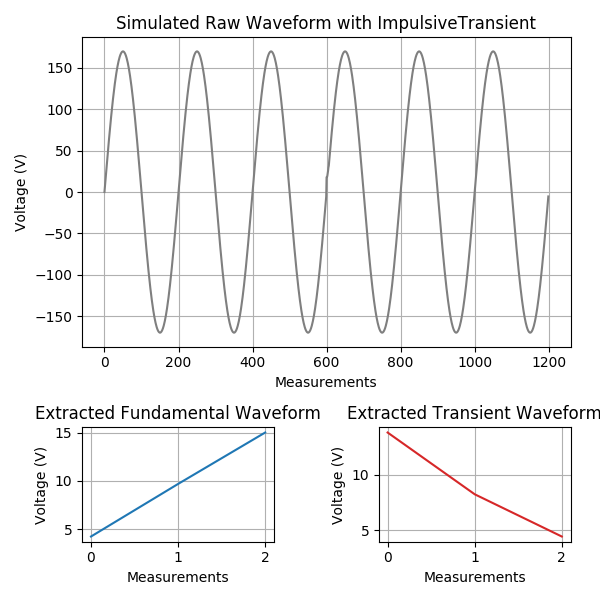
\includegraphics[scale=0.35]{./figures/impulsive_sim.png}
\caption{Simulated $60$ Hz $120$ Vrms sine wave with an impulsive transient. The decomposed fundamental and transient signal are shown in the bottom left and right subfigures, respectively.}\label{fig:ImpulsiveSim}
\end{figure}

Second, we created a simulated waveform with an oscillatory transient by superimposing an exponentially decaying sinusoidal wave with $960$ Hz frequency with starting amplitude of $72$ volts onto a portion of $6$ cycles of a fundamental waveform. The raw signal is shown in Figure \ref{fig:OscillatorySim}.

\begin{figure}[ht]
\centering%
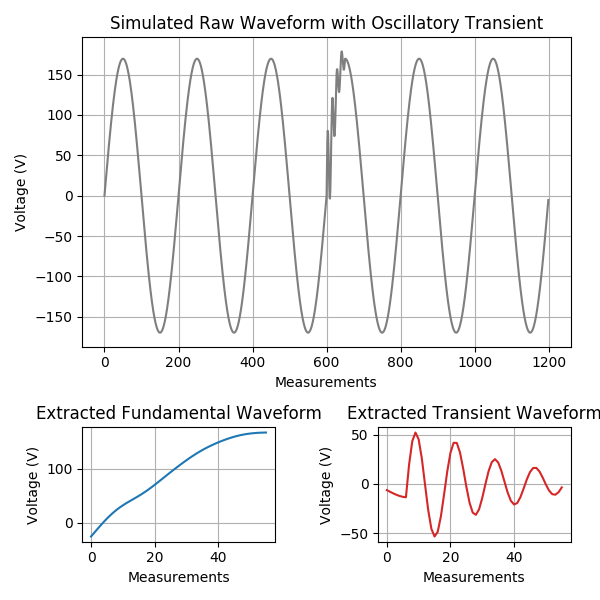
\includegraphics[scale=0.35]{./figures/oscillatory_sim.png}
\caption{Simulated $60$ Hz $120$ Vrms sine wave with an oscillatory transient. The decomposed fundamental and transient signal are shown in the bottom left and right subfigures, respectively.}\label{fig:OscillatorySim}
\end{figure}

Third, we created a simulated arcing transient by drawing 7 random samples from a uniform random distribution over the support $(61, 2401)$. We then used the random samples to define the frequencies for single cycles of an arcing transient wave. The raw signal is shown in Figure \ref{fig:ArcingSim}.

\begin{figure}[ht]
\centering%
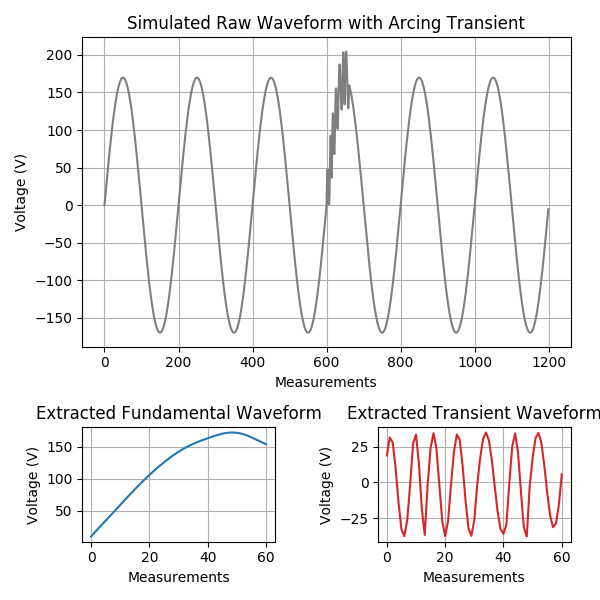
\includegraphics[scale=0.35]{./figures/arcing_sim.png}
\caption{Simulated $60$ Hz $120$ Vrms sine wave with an arcing transient. The decomposed fundamental and transient signal are shown in the bottom left and right subfigures, respectively.}\label{fig:ArcingSim}
\end{figure}


We simulated a multiple zero crossing transient by superimposing three single sawtooth cycles in positions of the fundamental waveform near a zero crossing. The single sawtooth cycle has an amplitude of a $72$ volts and a period of $10$ samples. The raw signal is shown in Figure \ref{fig:MultZSim}.

\begin{figure}[ht]
\centering%
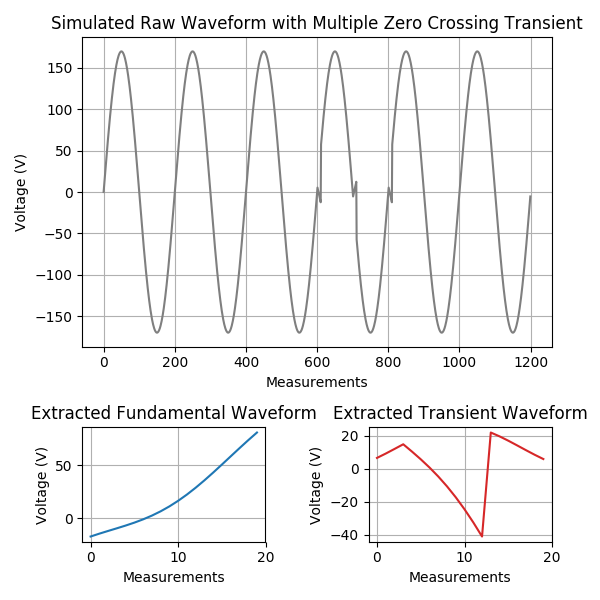
\includegraphics[scale=0.35]{./figures/mult_z_crossing_sim.png}
\caption{Simulated $60$ Hz $120$ Vrms sine wave with multiple impulsive transients which cause additional zero crossings in the raw waveform. The first decomposed fundamental and transient signal are shown in the bottom left and right subfigures, respectively.}\label{fig:MultZSim}
\end{figure}

Finally, we created a simulated waveform with a periodic notching transient by superimposing a sawtooth waveform with a frequency of $1440$ Hz and amplitude of $18$ volts for a single fundamental cycle, i.e., 24 notches per cycle for one cycle. We determined the polarity of the notching transient by the fundamental signal since notching is defined to be strictly negative in power. The raw signal is shown in Figure \ref{fig:NotchingSim}

\begin{figure}[htbp]
\centering%
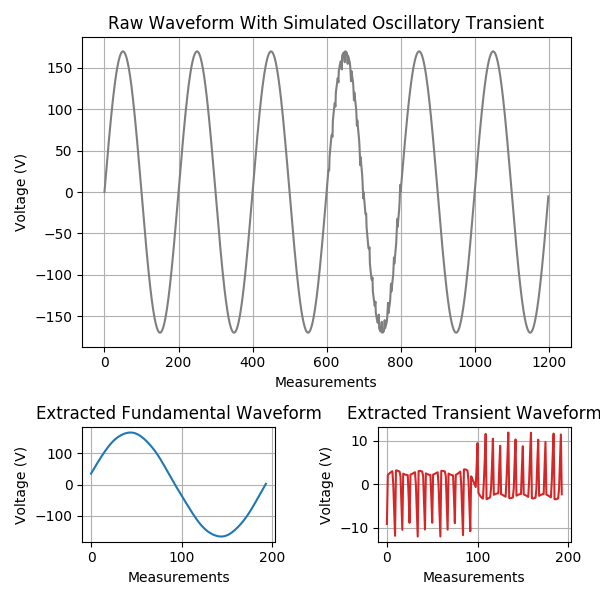
\includegraphics[scale=0.35]{./figures/notching_sim.png}
\caption{Simulated $60$ Hz $120$ Vrms sine wave with a periodic notching transient. The decomposed fundamental and transient signal are shown in the bottom left and right subfigures, respectively.}\label{fig:NotchingSim}
\end{figure}

Figures \ref{fig:ImpulsiveSim}, \ref{fig:OscillatorySim}, \ref{fig:ArcingSim}, \ref{fig:NotchingSim} show the raw simulated waveforms with impulsive, oscillatory, arcing, and periodic notching transients, respectively, all starting near the $600^{th}$ measurement. The two subfigures show the extracted fundamental waveform and transient waveform detected by the system. These simulated waveforms were all correctly classified by the system using our methods. 

\section{Conclusion and Future Work}
\label{sec:Conlcusion}

This paper presents an implementation of a transient detection system using OPQ, an open source distributed power quality network, which can successfully classify four types of transients as defined in the IEEE 1159 standard. Our method shows promise based upon its ability to correctly classify simulated versions of all four transients.

The most immediate future work is to monitor an electrical grid in real-time to determine how well the methods work on real world transients.

We also hope to add functionality to OPQ that would enable us to search our historical data for the occurrence of transients and classify them. From this, a meta-analysis for higher level network wide events could lead to clues regarding the sources of these phenomena. This data could provide new insight into our understanding of how intermittent renewable energy sources affect power quality on the grid, helping us to better modernize our grids with larger amounts of distributed renewable energy.


% conference papers do not normally have an appendix

% trigger a \newpage just before the given reference
% number - used to balance the columns on the last page
% adjust value as needed - may need to be readjusted if
% the document is modified later
%\IEEEtriggeratref{8}
% The "triggered" command can be changed if desired:
%\IEEEtriggercmd{\enlargethispage{-5in}}

% references section

% can use a bibliography generated by BibTeX as a .bbl file
% BibTeX documentation can be easily obtained at:
% http://www.ctan.org/tex-archive/biblio/bibtex/contrib/doc/
% The IEEEtran BibTeX style support page is at:
% http://www.michaelshell.org/tex/ieeetran/bibtex/
%\bibliographystyle{IEEEtran}
% argument is your BibTeX string definitions and bibliography database(s)
%\bibliography{IEEEabrv,../bib/paper}
%
% <OR> manually copy in the resultant .bbl file
% set second argument of \begin to the number of references
% (used to reserve space for the reference number labels box)
%
% As suggested below, edit bibtemplate_samples.bib to reflect
% your bibliography. See bibtemplate.text for referencing.
%

\bibliographystyle{IEEEtran}
\bibliography{references}

% that's all folks
\end{document}


